\documentclass[conference]{IEEEtran}
\IEEEoverridecommandlockouts
% The preceding line is only needed to identify funding in the first footnote. If that is unneeded, please comment it out.
\usepackage{cite}
\usepackage{amsmath,amssymb,amsfonts}
\usepackage{algorithmic}
\usepackage{graphicx}
\usepackage{textcomp}
\usepackage{xcolor}
\def\BibTeX{{\rm B\kern-.05em{\sc i\kern-.025em b}\kern-.08em
    T\kern-.1667em\lower.7ex\hbox{E}\kern-.125emX}}
\begin{document}

\title{Item-based Filtering Enhanced by SVD\\
}

\author{\IEEEauthorblockN{Ali Eren Çiftçi}
\IEEEauthorblockA{\textit{Istanbul Technical University} \\
Istanbul, Turkey \\
ciftcia22@itu.edu.tr}
}

\maketitle

\begin{abstract}
In this paper, we focus on the Singular Value Decomposition (SVD) method developed with the item-based filtering technique. Item-based filtering is a method that recommends items with similar characteristics based on users' past preferences. SVD is a matrix factorization technique used to identify hidden relationships in large-scale datasets.
\end{abstract}

\section{Introduction}
Nowadays, in online platforms and digital media environments, it has become an important need to recommend content that matches users' interests. Especially in movie and TV series platforms, being able to offer content according to users' tastes increases both user satisfaction and the effectiveness of the platform. In this context, recommendation systems have gained great importance. The main goal of this study is to combine item-based filtering with traditional SVD to more accurately predict users' movie preferences and provide more personalized movie recommendations. This will not only enhance the user experience, but also provide platform owners with more effective content management and user loyalty.

\section{Background}

\subsection{Singular Value Decomposition (SVD) }

Singular Value Decomposition (SVD) is a linear algebra technique for decomposing matrices. It represents a matrix as the product of three smaller and more specialized matrices: a right-order matrix, a diagonal matrix and a left-order matrix. This matrix decomposition is useful for discovering hidden relationships. In particular, in large datasets, SVD can be used to understand hidden structure, reducing data size, and identifying features. \\
Mathematically, a matrix $A$ of size $m \times n$ can be decomposed using Singular Value Decomposition (SVD) into three components:

\[ A = U \Sigma V^T \]

Here, \\
- $U$ is an $m \times m$ orthogonal matrix, \\
- $\Sigma$ is an $m \times n$ diagonal matrix containing the singular values arranged in descending order, \\
- $V$ is an $n \times n$ orthogonal matrix.\\

SVD allows for the compression of information by reducing the dimensionality of the matrix and revealing hidden relationships within the dataset. Particularly, by selecting $k$ singular values, an approximation $A_k$ of the original matrix $A$ can be obtained. This approximation is calculated using the columns and rows corresponding to the top $k$ singular values:

\[ A_k = U_k \Sigma_k V_k^T \]

Here, $U_k$, $\Sigma_k$, and $V_k$ are submatrices consisting of the first $k$ columns of $U$, $\Sigma$, and $V$, respectively.

SVD can be utilized in recommendation systems to provide recommendations based on user-item interactions. By representing user preferences in a matrix form, SVD can uncover the latent structure within the data, enabling predictions of future preferences.

\subsection{Item-Based Collabrative Filtering}

Item-based collaborative filtering is a recommendation technique that suggests items to users based on the similarity between items. In this approach, the similarity between items is measured, typically using metrics such as cosine similarity or Pearson correlation coefficient. The basic idea is to recommend items that are similar to those that a user has liked or interacted with in the past.

For example, consider a movie recommendation system. If a user has rated or liked certain movies, item-based collaborative filtering identifies other movies that are similar to the ones the user has enjoyed. The similarity between movies can be determined based on factors such as genre, cast, director, or user ratings.

One advantage of item-based collaborative filtering is its scalability. It can handle large datasets efficiently, as the similarity between items is precomputed and stored in a similarity matrix. Additionally, it is robust to new items being added to the system, as the similarity between items can be updated incrementally without recalculating all similarities.

Overall, item-based collaborative filtering provides personalized recommendations by leveraging the similarity between items, enabling users to discover new items that match their interests based on their past interactions.


\section{Implementing Item-Based Collaborative Filtering Algorithm with Python}

\textbf{Introduction:}

For implementation in Python, we can utilize libraries such as \texttt{json}, \texttt{numpy}, \texttt{pandas}, and \texttt{matplotlib}.\\

\textbf{1. Loading the Dataset (\texttt{json}):} The first step is to load a dataset that represents user-item interactions. This dataset is typically stored as a JSON file and contains information such as user ratings or interaction types.

\textbf{2. Processing the Dataset (\texttt{pandas}, \texttt{numpy}):} We can use the \texttt{pandas} library to process the loaded dataset. By converting the dataset into a DataFrame, we can create the user-item matrix. Then, we can perform matrix operations using the \texttt{numpy} library.\\

\textbf{3. Calculating Item Similarities (\texttt{numpy}):} To compute similarities between items, we can use the \texttt{numpy} library. For example, we can calculate cosine similarity using vector operations provided by \texttt{numpy}.\\

\textbf{4. Generating User Recommendations:} Once the item similarities are calculated and the recommendations are made, we can evaluate the performance of our recommendation system. One common metric for evaluating recommendation systems is the Mean Absolute Error (MAE), which measures the average absolute difference between the predicted ratings and the actual ratings given by users.

To visualize the MAE, we can use the \texttt{matplotlib} library. We can plot the MAE values over iterations or other relevant factors to observe how the recommendation system's performance changes over time or with different parameters.

The following steps outline how to visualize MAE using \texttt{matplotlib}:\\
1. Compute MAE: Calculate the MAE values for different iterations or parameter settings.\\
2. Plot MAE: Use \texttt{matplotlib} to create a line plot or a bar plot showing the MAE values over iterations or parameter settings.\\
3. Interpret Results: Analyze the plot to understand how the MAE changes and whether the recommendation system's performance improves or deteriorates under different conditions.\\

By visualizing the MAE, we can gain insights into the effectiveness of our item-based collaborative filtering algorithm and make informed decisions about its optimization and fine-tuning.


\textbf{5. Experimental Setup and Code Implementation}
In our experimental setup, we utilized the IMDb dataset, which provides movie ratings on a scale of 1 to 10. To ensure the reliability of our recommendations, we focused on reviewers who have rated at least 20 films. By selecting this subset of reviewers, we aimed to include users with a sufficient number of ratings to provide meaningful insights into their preferences and tastes.

The IMDb dataset offers a rich source of movie ratings contributed by a diverse range of users. By leveraging this dataset, we were able to develop and implement an item-based collaborative filtering algorithm in Python. This algorithm analyzes the similarities between movies based on the ratings provided by users and generates personalized recommendations for each user.

In this section, we will outline the experimental setup, including the preprocessing steps applied to the IMDb dataset, the implementation of the item-based collaborative filtering algorithm using Python, and the evaluation metrics used to assess the performance of our recommendation system. Additionally, we will discuss the insights gained from the experiments and the implications of our findings.

\subsection {Algorithm}

\begin{itemize}
\item First construct the matrix (reviewer, movie). In the cells of the matrix we write the reviewer's rating for the movie.
\item Then we find the average of each row and column of this matrix to fill the empty elements of this matrix. Then add to each cell the average of the column it is in and subtract the row average.
\item Then we apply SVD to this matrix with the help of the QR algorithm. And reduce the SVD result by selecting k singular values. Let's call this matrix $R_{red}$. And calculate $\sqrt{E_k}V^T_k$ to get our meta ratings matrix.
\item  Let's do an adjusted cosine similarity calculation using the meta ratings matrix and note the movies with the highest L score.
\item Finally, let's find the Prediction Generation result using the similarity result, the $R_{red}$ matrix, and the row averages of these L movies.
\end{itemize}

\subsection {MAE}
At this stage, MAE was calculated using L = [20,60,80], k = [2,4,6,8,10,20]. First, MAE is calculated for 5 users individually. For example, the graphs of the $1^{st}$ user are as follows. The common result for these 5 users is that k gives a minimum MAE of 6-8 and L gives a minimum MAE of 20. However, the average MAE was 0.05 for one user but 0.95 was for all users. This result is due to the different ratings given by users to similar movies. This is, of course, something that can happen in life, so taking into account all users, the MAEs of each user for each (k,L) pair are found and then these MAEs are averaged and the result is as follows.
\begin{figure}[htbp]
\centerline{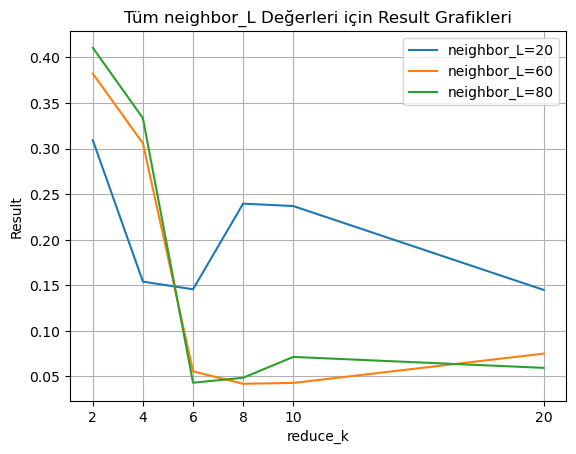
\includegraphics[scale = 0.5]{user1.png}}
\caption{User 1}
\label{fig}
\end{figure}
\begin{figure}[htbp]
\centerline{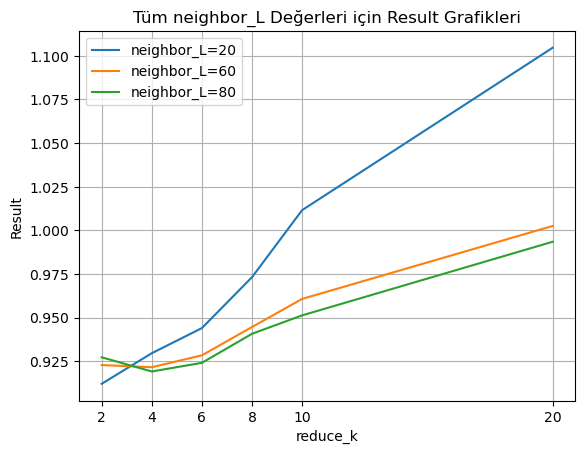
\includegraphics[scale = 0.5]{user_all.png}}
\caption{All users}
\label{fig}
\end{figure}


Looking at all users, the minimum MAE is k = 4. The result of MAE at this value is 0.95. Therefore, our algorithm can predict a user's rating of a movie at $\pm9.5$. 

\section{Conclusion and Future Work}

In this paper, an item-based algorithm augmented with SVD is tested. SVD is used to find the meta ratings matrix. This reduces the error in similarity detection and prediction. Thanks to these benefits of SVD, predictions can be made with a deviation of around $\pm0.5\%$. This result is quite sufficient for a movie recommendation application.




\begin{thebibliography}{00}
\bibitem{b1} Vozalis, M. G., Margaritis, K. G. (2007). Using SVD and demographic data for the enhancement of generalized Collaborative Filtering. Information Sciences, 177(15), 3017–3037.
\end{thebibliography}


\end{document}
